\documentclass{article}

\usepackage[final]{nips_2018}

\usepackage[utf8]{inputenc} % allow utf-8 input
\usepackage[T1]{fontenc}    % use 8-bit T1 fonts
\usepackage{hyperref}       % hyperlinks
\usepackage{url}            % simple URL typesetting
\usepackage{booktabs}       % professional-quality tables
\usepackage{amsfonts}       % blackboard math symbols
\usepackage{nicefrac}       % compact symbols for 1/2, etc.
\usepackage{microtype}      % microtypography
\usepackage{float}
\usepackage{natbib}
\usepackage{graphicx}
\usepackage{subfigure}
\usepackage{booktabs}

\usepackage{color}

\bibliographystyle{plainnat}
\setlength{\parskip}{0pt}

\def\defeq{\dot=}

\title{Analyzing the Role of Temporal Differencing in Deep Reinforcement Learning}

\author{
  Alexandre Beaulne \\
  \texttt{alex@mgnr.io} \\
  ID 20087309
  \And
  Amina Madzhun \\
  \texttt{amina.madzhun@umontreal.ca} \\
  ID 20052277
}

\begin{document}

\maketitle
\section{Introduction}

Our project has for objective to reproduce a subset of
the results from TD or Not TD: Analyzing the Role of Temporal
Differencing in Deep Reinforcement Learning \citep{amiranashvili2018analyzing}.
In recent years, techniques combining Reinforcement Learning (RL)
and Deep Learning (DL) have emerged \citep{mnih2015} to produce
superhuman performance at some control tasks. However, the behavior
of deep neural architectures when used as function approximators
in RL is still poorly understood. The chosen paper aims to improve
this understanding.

\subsection*{Background}

RL is an area of machine learning concerned with how software agents
ought to take actions in an environment so as to maximize some notion
of cumulative reward \citep{suttonbarto2018}. In the traditional RL
framework, an agent's evolution is \emph{entirely} defined by a sequence
of state, action and reward tuples. This sequence forms a
partially observable Markov decision process (POMDP). The objective
of the agent is to pick the action in any state that will
maximize the cumulative rewards encountered till the end of the
sequence (the \emph{episode}).\\

More rigorously, a standard RL problem develops over discrete
time steps involving an episodic setup (starting an episode at
$t=0$ and finishing it at terminal time step $t=T$).
The agent evolves in a stochastic environment with its current state
$s_t$ at time step $t$, and can can perform an action $a_t$ from a
set of actions. This action leads the environment to a new state
$s_{t + 1}$, and gives a reward $r_t$ to the agent or finishes the episode.
The goal of the agent is to learn a policy $\pi(a_t|s_t)$
to obtain the maximum expected return over time which is
the total amount of reward that it can get from the current time step
to the end of the episode, with future rewards being reduced by discount
factor $\gamma$ for each time step. \\

For a given policy $\pi$ the value function and the action-value function
are defined as:
    \begin{eqnarray*}
    V^\pi(s_t) \defeq \mathbb{E}_{\pi} [\hat{R}_t | s_t], &
    Q^\pi(s_t, a_t) \defeq \mathbb{E}_{\pi} [\hat{R}_t | s_t, a_t]
    \end{eqnarray*}
where $\hat{R}_t$ is cumulated discounted reward

\begin{equation}
R^\gamma_t = \sum_{i=t}^T \gamma^{i-t} r_i
\end{equation}

or a truncated sum

\begin{equation}
R^\tau_t = \sum_{i=t}^{t+\tau} r_i
\end{equation}

$\tau$ in this case is a fixed number of steps; the \emph{horizon}.

The optimal state and state-action value functions are respectively given by

\begin{eqnarray} \label{optimal}
    V^*(s_t) \defeq \max_{\pi}V^\pi(s_t), &
    Q^*(s_t, a_t) \defeq \max_{\pi} Q^\pi(s_t, a_t)
\end{eqnarray}

Value based algorithms to find the optimal policy require computing
or approximating one of the value function from equation (\ref{optimal}).

\section{Paper Summary}
RL algorithms to find optimal policies involve exploring trajectories
and backtracking observed rewards to previous visited state-action pairs.
The depth and breath of the search vary between different algorithms
(Figure (\ref{backups})).

\begin{figure}[H]
    \centering
    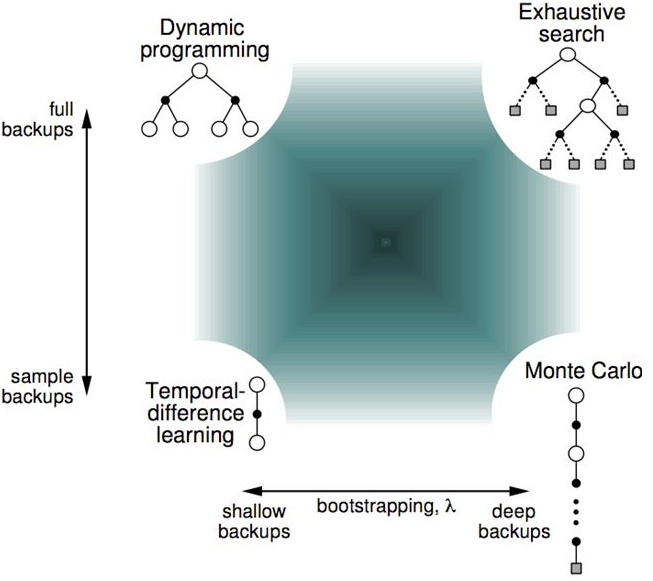
\includegraphics[scale=0.35]{backups}
    \caption{Different backtracking schemes \citet{suttonbarto2018}}
    \label{backups}
\end{figure}

The large size of the state space of the problems considered preclude full breadth
search, which leaves sampling as the only viable exploration scheme. Sampling
search can be divided into two approaches, depending on the depth of the trajectory
sampled. Monte Carlo (MC) search samples a trajectory till the end, while temporal
differencing (TD) samples a single step, and approximate the value of the rest of the
trajectory with the current value function at the next state (i.e. \emph{bootstrap}).
Naturally, the complete spectrum of hybrid exploration depths, i.e. rollout length,
from 1 step (TD) to the end of the episode (MC) is possible.
Before the advent of deep network as function approximators, it has been empirically
demonstrated that TD is superior to MC \citep{sutton1995}. However, it is unclear
whether those results still hold with the use of deep neural nets as function approximators.
This question is explored in \citep{amiranashvili2018analyzing}. \\

The authors perform two sets of experiments. In one set, they benchmark three different
algorithms (A3C, n-step Q-learning and $Q_{MC}$) on games from the Atari and VizDoom environments,
varying rollout lengths. The second set of experiments are \emph{controlled}, fixed algorithms
were tested against environments whose reward randomness, delay and sparsity were
carefully adjusted.\\

They conclude that MC estimation is a feasible and sometimes even competitive alternative
to TD. MC performs particularly well in visually complex 3D environments
and with delayed or sparse rewards. As for rollout, the authors obtain the
best results with a rollout length of 20.

\begin{table}[H]
\centering
\label{table1}
    \begin{tabular}{@{}l|c|cc}
    \toprule
                                             & \#steps  & Seaquest  & Pong  \\ \midrule
    20-step A3C (Mnih et al., 2016)          & 80M      & 2300      & 11.4  \\ \midrule
    $Q_{MC}$ (Amiranashvili et al., 2017)    & 60M      & 12708     & -4.2  \\
    20-step $Q$ (Amiranashvili et al., 2017) & 60M      & 4276      & 8.9   \\
    20-step A3C (Amiranashvili et al., 2017) & 60M      & 2021      & 20.6  \\ \midrule
    20-step $Q$ (our results)                & 20M      & 100       & 21    \\
    20-step A3C (our results)                & 20M      & 2702      & 21    \\ \bottomrule
    \end{tabular}
\caption{Our results at two Atari games against selected publications. Higher scores are better for both games.}
\end{table}

\begin{figure}[H]
    \centering
    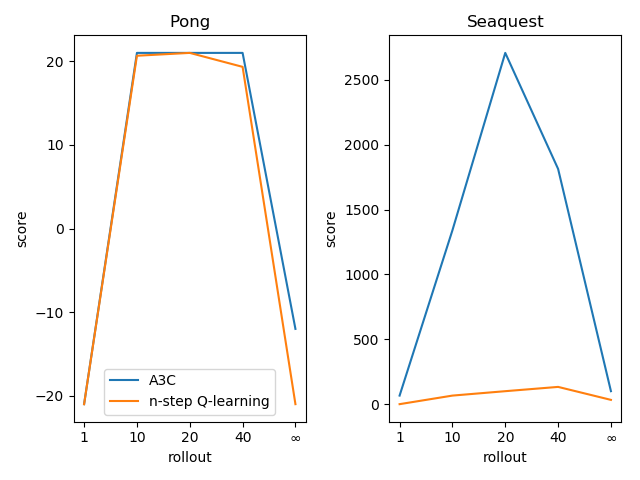
\includegraphics[scale=0.75]{results}
    \caption{Effect of rollout length on TD learning for n-step Q and A3C. Score on
    Pong and Seaquest Atari games. Higher is better.}
    \label{rollouts}
\end{figure}


\pagebreak


\subsection{Motivation}
% - What are the motivation and problem? Give some background.
In RL setup numerous results in the past have proven
that for low-dimensional feature representations and linear function
approximators Temporal Difference learning outperforms
Monte Carlo estimation. However, in deep RL the spectrum of problems
has been broadened by using deep network architectures for function
approximation. This allowed to handle high dimensionality inputs,
extremely large state space and more sophisticated environments with partial
observability, still TD serves as the basis for
most of developed algorithms. One of the problems in deep RL is that
the choice of algorithm for given task is based on empirical results.

\subsection{Proposed approach}
% - How do they propose to solve it?
\color{red}
The more complicated model architectures become with developing
new solutions, the more serious becomes the issue of defining causes
for perplexing performance
or the correctness of results.
To surpass potential mistakes in conclusion for an analysis of algorithms,
the authors try to separate the factors which could influence
the performance:
\begin{enumerate}
\item complexity of the environment  \\
Experiments on 1D to 3D environments
\item algorithm configurations \\
Consider three essential aspects:
\begin{itemize}
  \item TD or MC (infinite) varying rollout length in the
  update, -> n-step Q learning
  \item infinite vs finite horizon -> Q\_MC
  \item pure based vs A3C not to be limited in conclusions -> A3C from Mnih
\end{itemize}
\item environment properties \\
consider different factoring by criterias: sparse, delayed rewards, terminal
state, reward type, perceptual complexity
\end{enumerate}

+ additional help/observations in terms of health gathering<...> problems

\color{black}

\section{Experiments}
% Discuss the experiments conducted in the paper. A good way to go about doing this is to think about what the advantages of the model are, and what might be a good way to demonstrate that before looking at what was attempted by the authors.

% - What are the authors trying to demonstrate with the experiments?

 \textcolor{red}{describe controlled experiments, VizDoom environments, perception}

% - Are there experiments that might demonstrate weaknesses/strengths that should be there but aren’t?
% - Are there any flaws in the experiments they run? What are they?
% \textcolor{red}{paper review comments}
% 	https://openreview.net/forum?id=HyiAuyb0b

\subsection{Motivation for the experiments}
\subsection{Reproducing the main results}
% Reproducing the results. Apart from the experimental details included in the paper, you should also include details that were not included.
% - What are some of the hyperparameters that were excluded from the paper? How important were they to get things working?
% - Are there technical details (missing or wrong equations, etc.) that were missing from the paper? If yes, what were they and what did you do to fill in the gap. Justify your choices.



\section{Discussion}
% - How is the experiment aligned with proposed approach/analysis
% - Criticism of missing information, unmentioned drawbacks (if any)


\citet{mnih2015} \\
OpenAI's Gym \citep{gym} \\
\citep{pytorch} \\
\citet{amiranashvili2018analyzing} \\
\citet{pmlr-v48-mniha16}

\pagebreak

\small

\bibliography{main}

\end{document}

